\documentclass[11pt]{article}
\usepackage[font=small]{caption}
\usepackage[margin=1in]{geometry}
\usepackage{amsmath, amssymb}
\usepackage{graphicx}
\usepackage{booktabs}
\usepackage[hidelinks]{hyperref}
\usepackage{microtype}

\title{Spatiotemporal Electricity Price Modeling and Stochastic Battery
Dispatch:\\ a Neural Jump-Diffusion and Deep BSDE Study on CAISO Data}
\author{Manthan Acharya}
\date{August 2026}

\begin{document}
\maketitle

\begin{abstract}
Locational electricity prices diverge because power flows obey physics:
when a transmission line reaches its thermal limit, the marginal cost of
serving load splits by location. This paper builds a battery dispatch
policy that conditions on those location spreads and checks each modeling
layer on its own before the next one uses it. A DC optimal power flow on a synthetic IEEE 14-bus network
reproduces congestion pricing; a neural jump-diffusion fit to eighteen months of
real CAISO hub prices supplies the dynamics; dispatch is solved as
four-dimensional stochastic control with a deep BSDE solver
\cite{weinan2017,han2018}, cross-checked against grid dynamic programming;
and the policy is backtested on realized 2026 prices. The policy captures 88.5\% of
the perfect-foresight benchmark (95\% CI 84.8--92.6). A fixed hour-of-day
schedule captures 87.5\%, and the 1.0-point gap between them (95\% CI
$-2.6$ to $+4.5$) is indistinguishable from zero. The price model
reproduces spike frequency and the first two moments within pre-registered
tolerances and beats a seasonal Ornstein--Uhlenbeck baseline on held-out
likelihood. It still fails a block-bootstrap KS test, a rank-histogram test
shows it biased high, and its half-life check passes or fails depending on
the simulation seed. The deep BSDE disagrees with dynamic programming at
three of sixty test states. Four further variants of the price model
improved individual diagnostics, and none passed every goodness-of-fit
check.
\end{abstract}

\section{Introduction}

Grid-scale batteries generate revenue primarily through temporal arbitrage:
charging when electricity is cheap and discharging when it is expensive \cite{sioshansi2009}.
The usual evaluation optimizes against a point forecast of one aggregate
price, which leaves out two things.

First, electricity prices are locational. The same megawatt-hour
trades at different prices across network locations whenever a
transmission constraint binds, and these spreads reveal the physical state of
the grid. A battery sited at a given location should condition on the joint state
of neighboring prices as well as its own.

Second, stored energy is an option. A battery holding
50~MWh at noon holds the right to sell into the evening peak; the value of this right
depends on the full conditional distribution of future prices, including spike dynamics,
mean-reversion rates, and negative midday prices. Valuing and exercising this option
requires solving a continuous stochastic control problem: at each decision epoch,
the optimal action depends on the conditional marginal value of stored energy.

This paper addresses both on real market data. It (i) works through
spatial price divergence on a synthetic grid model, (ii) fits a
continuous-time jump-diffusion to three CAISO hub LMPs, (iii) solves the
control problem with a deep BSDE solver checked against dynamic programming,
and (iv) backtests the policy on realized prices.

\section{Power pricing theory}

Electricity is not storable at scale, so supply must equal demand at every
instant at every location, and the price of the marginal megawatt is set
by whichever generator would serve one more unit of load at that
location, right now.

\subsection{Nodal pricing}
Modern US markets settle at locational marginal
prices (LMPs): the cost of serving one additional MW at each network node,
computed from a security-constrained optimal power flow, meaning the
least-cost dispatch of all generators subject to the physical limits of
the network \cite{schweppe1988}. Each LMP
decomposes into a system-wide energy component, a congestion component
(the shadow prices of binding transmission constraints, spread across
locations by the network's sensitivities), and a small loss component.
When network constraints are slack, nodal prices coincide; when transmission lines bind,
prices diverge according to network topology and line sensitivity factors
(Section~\ref{sec:grid}).

\subsection{Stylized facts}
Because demand is inelastic on hourly timescales
and supply stacks are steep at the margin, power prices behave unlike
other asset classes \cite{lucia2002,cartea2005}: they are strongly
mean-reverting (a scarcity hour does not imply scarcity tomorrow),
strongly seasonal on daily and weekly clocks, spiky (hourly moves of many
standard deviations), and, in solar-heavy systems, frequently
negative, when must-run and subsidized generation exceeds midday
demand. California is the clearest case: solar pushes midday prices low or
negative, and a steep ramp follows at sunset. A model used to value
storage has to reproduce these facts, because storage earns its revenue
from the daily valley-to-peak swing and its uncertainty.

\subsection{The 2025--26 CAISO regime}
The data period studied here has a
further feature: California's rapidly grown battery fleet now flattens the
evening peak. Hub-level day-ahead prices stay within roughly $-\$43$ to
\$150/MWh over the whole eighteen months; the fat tails are in the hourly
increments (excess kurtosis 7--9), and
negative hours are common (5--15\% by hub). The level also moved: February--March
hub means fell by about a quarter between 2025 and 2026 and their standard
deviations by about 40\%, and the April--June 2026 test quarter averages
60\% below the training split, a shift any model fitted on 2025 has to
survive.

\section{Physical grid model}
\label{sec:grid}

The grid layer exists to demonstrate, in a controlled setting, the
mechanism that produces the spreads the price model later conditions on.
The topology is synthetic and its economics are constructed: the
standard IEEE 14-bus test case \cite{christie1993}, with distinct linear
generator costs (15/30/40/45/50 \$/MWh) assigned to its five generators
and a single 190~MW thermal limit imposed on the line from bus~1 to
bus~2, chosen so the limit is slack at base load and binds under a
$+40$~MW perturbation at bus~3. Nothing computed on this network is
fitted to, or calibrated against, the CAISO price data; the real WECC
topology is not public at network-model fidelity, so the network is used
only to show how the LMP decomposition works.

Under the DC approximation (dominantly inductive lines, flat voltage
magnitudes, small angles), the flow on line $l$ from bus $i$ to $j$ with
reactance $x_l$ is $f_l = (\theta_i - \theta_j)/x_l$; collecting lines
into the incidence matrix $A$ and $B_d = \mathrm{diag}(1/x_l)$, nodal
injections satisfy
\begin{equation}
P = A^\top B_d A\,\theta =: B\theta, \qquad f = B_d A\,\theta .
\label{eq:dcflow}
\end{equation}
Fixing a slack bus and inverting the reduced $\tilde B$ yields the power
transfer distribution factors (PTDFs)
\begin{equation}
H = B_d A\, \tilde B^{-1}_{\uparrow}, \qquad
H_{l,k} = \partial f_l / \partial P_k,
\label{eq:ptdf}
\end{equation}
the sensitivity of every line flow to injection at every bus. The market
dispatch is the linear program
\begin{equation}
\min_{p}\; c^\top p \quad \text{s.t.}\quad
\mathbf{1}^\top p = \mathbf{1}^\top d \;(\lambda), \qquad
-\bar f \le H(M_g p - d) \le \bar f \;(\mu^\mp), \qquad
0 \le p \le p^{\max},
\label{eq:dcopf}
\end{equation}
and differentiating its Lagrangian with respect to nodal demand gives the
LMP decomposition
\begin{equation}
\mathrm{LMP}_k \;=\; \lambda_{\text{sys}} \;-\; \sum_{l \in \text{lines}} \big(\mu^+_l - \mu^-_l\big)
H_{l,k} \;=\; \lambda_{\text{sys}} + C_{k,\text{cong}},
\label{eq:lmp}
\end{equation}
energy plus congestion (the DC model is lossless, so the loss term of the
industry decomposition is identically zero here).

The PTDF implementation reproduces
the classic three-bus equal-reactance example exactly ($2/3$ of an
injection takes the direct path, $1/3$ the two-hop path) and matches
pypower's independent \texttt{makePTDF} on case14 \cite{thurner2018} to
$9\times10^{-16}$ once off-nominal transformer tap ratios are included;
without them the flows are off by order $10^{-2}$. The congestion
experiment (Figure~\ref{fig:congestion}) then shows the mechanism end to
end: at base load nothing binds and all fourteen buses price at
$\lambda = \$15$/MWh; after the perturbation the line binds with shadow
price $\mu = \$17.9$/MWh, prices fan out over a \$15/MWh range, and the
realized congestion component at every bus equals $-\mu H_{l,k}$ to
machine precision ($1.8\times10^{-15}$), with the sign of the price gap
matching the PTDF sign at all thirteen nonzero-PTDF buses.

\begin{figure}[tbp]
\centering
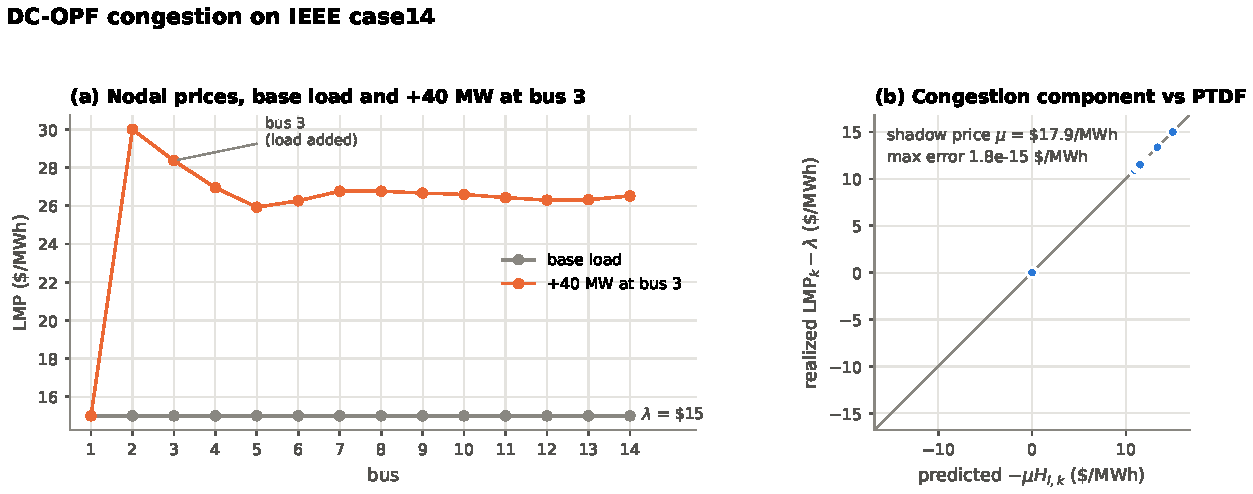
\includegraphics[width=0.92\textwidth]{figures/congestion_experiment.pdf}
\caption{Left: nodal prices on IEEE case14 before and after a $+40$~MW
load perturbation at bus~3 binds the 190~MW limit on line 1--2. Right:
realized congestion component versus the PTDF prediction $-\mu H_{l,k}$;
agreement is to machine precision.}
\label{fig:congestion}
\end{figure}

Hub spreads connect the grid model to real data through the identity $\mathrm{LMP}_i - \mathrm{LMP}_j =
(C_i - C_j) + (L_i - L_j)$: hub spreads are congestion differentials up to
small loss terms. On the CAISO data the NP15$-$SP15 spread and CAISO's own
published congestion differential correlate at $0.99$, with mean absolute
loss residuals of \$0.4--1.2/MWh against mean absolute spreads of
\$2--6.5/MWh. Spreads are therefore used as the observable congestion
state throughout the price model of Section~\ref{sec:sde}.

\subsection{Predictions tested against CAISO data}
\label{sec:gridlink}

The SDE cannot condition on DC-OPF shadow prices: the network is synthetic
while the prices are real, so case14's congestion prices bear no
statistical relation to CAISO's. Nor can it condition on CAISO's published congestion
component, which is exogenous: simulating forward would need future
congestion values, and the state would no longer be Markov. The grid layer instead supplies
falsifiable predictions about the shape of any DC-OPF congestion
field, tested against CAISO's own data (Figure~\ref{fig:gridlink}).

The first two predictions hold. Hourly spread innovations track CAISO congestion
innovations at $R^2 = 0.975$ and $0.985$. And the
congestion field is strongly low-rank: participation ratio 1.54 out of 3
(1.09 for case14; 3 would be isotropic), with a leading component
explaining 78.8\% of variance and loading $(-0.572,\,0.573,\,0.587)$.
That is a north-versus-south contrast, matching the Path-15 split: the
major transmission corridor separating northern from southern California,
and the constraint the NP15 and SP15 hubs take their names from.

The third does not. If congestion lived
on discrete PTDF rays, large events would be more directionally
concentrated than small ones; case14 collapses to a median angular
dispersion of $1.1^\circ$, but CAISO falls only from $48.6^\circ$ to
$25.7^\circ$ across deciles of congestion magnitude, against a
covariance-matched Gaussian null falling from $58.0^\circ$ to
$14.6^\circ$. CAISO is distinguishable from that null (decile drop
$22.9^\circ$ versus $43.4 \pm 0.6^\circ$, outside all 200 null draws) but
nowhere near the synthetic network's discrete PTDF rays. The sharp geometry of a 14-bus
network does not survive aggregation into three hub prices, where many
constraints across a large system superpose.

\begin{figure}[tbp]
\centering
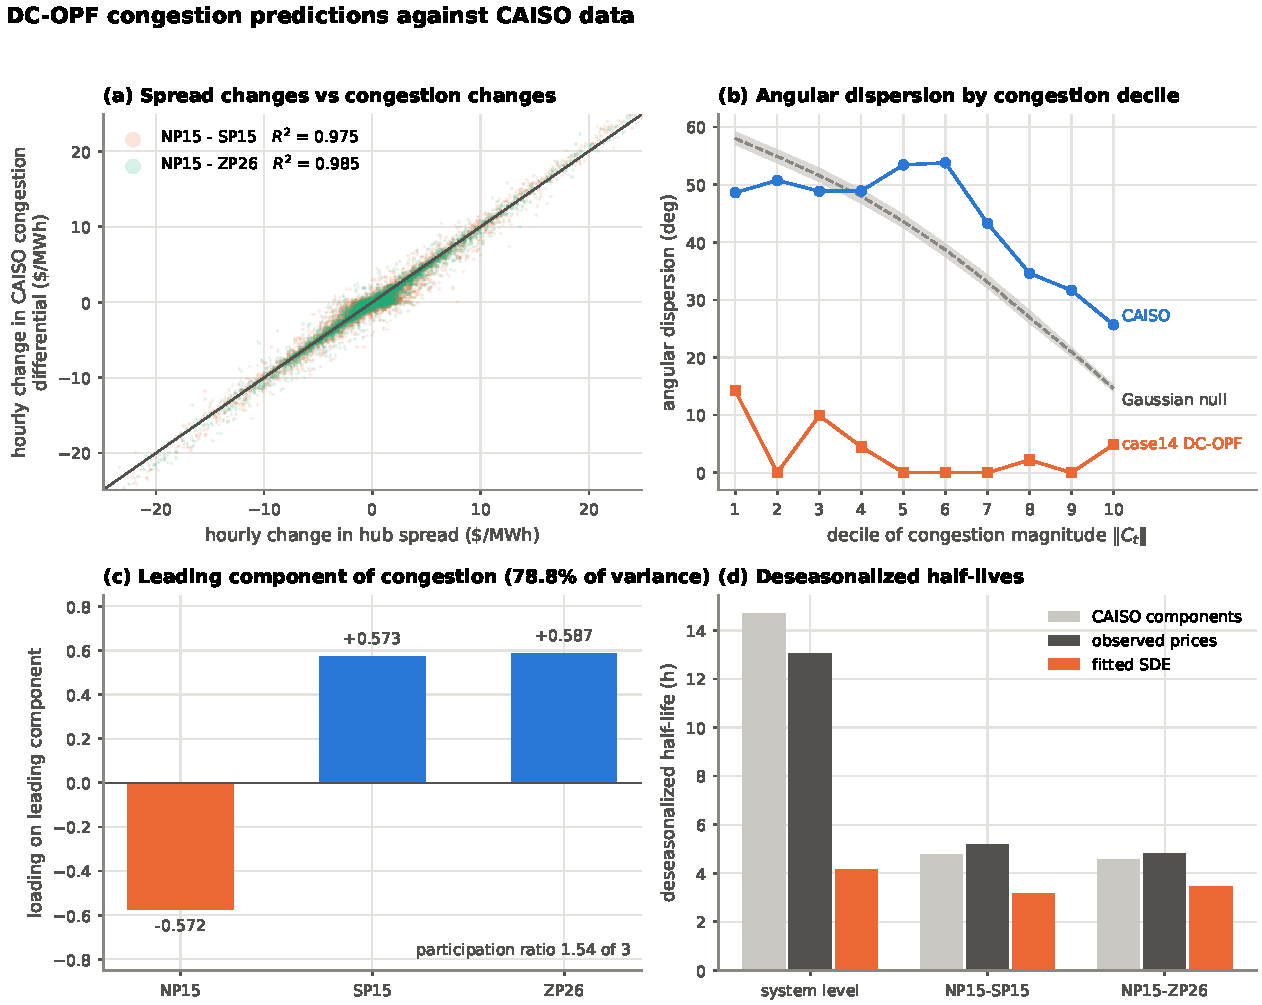
\includegraphics[width=\textwidth]{figures/congestion_link.pdf}
\caption{DC-OPF predictions tested on CAISO hub data. (a)~Hourly hub-spread changes against changes in CAISO's published congestion differential. (b)~Angular dispersion of the congestion vector by decile of its magnitude, for CAISO, a covariance-matched Gaussian null (mean and 95\% band over 200 draws) and the case14 field. (c)~Loadings of the leading principal component of the CAISO congestion field. (d)~Deseasonalized half-lives of the system level and the two spreads.}
\label{fig:gridlink}
\end{figure}

\section{Stochastic price dynamics}
\label{sec:sde}

\subsection{Data}
Eighteen months (January 2025 -- June 2026) of CAISO day-ahead hourly LMPs
for the three trading hubs NP15, SP15 and ZP26. A trading hub is an
aggregated pricing point averaging many physical nodes, and is what most
contracts actually settle against; the cost of that convenience is that
hub prices smooth away much of the nodal detail of
Section~\ref{sec:grid}. The series was pulled from OASIS via
\texttt{gridstatus}, cleaned to a gapless 13{,}103-hour record, and split
chronologically: train through January 2026, validation February--March
2026, test April--June 2026, with no shuffling. Figure~\ref{fig:data}
shows the series and a ten-day window in which NP15 trades \$20--30 above
the southern hubs for days at a time. Real-time 15-minute hub prices,
sampled over three 2025 windows, showed tails no heavier than day-ahead,
so the fourfold data volume was not worth taking on.

\begin{figure}[tbp]
\centering
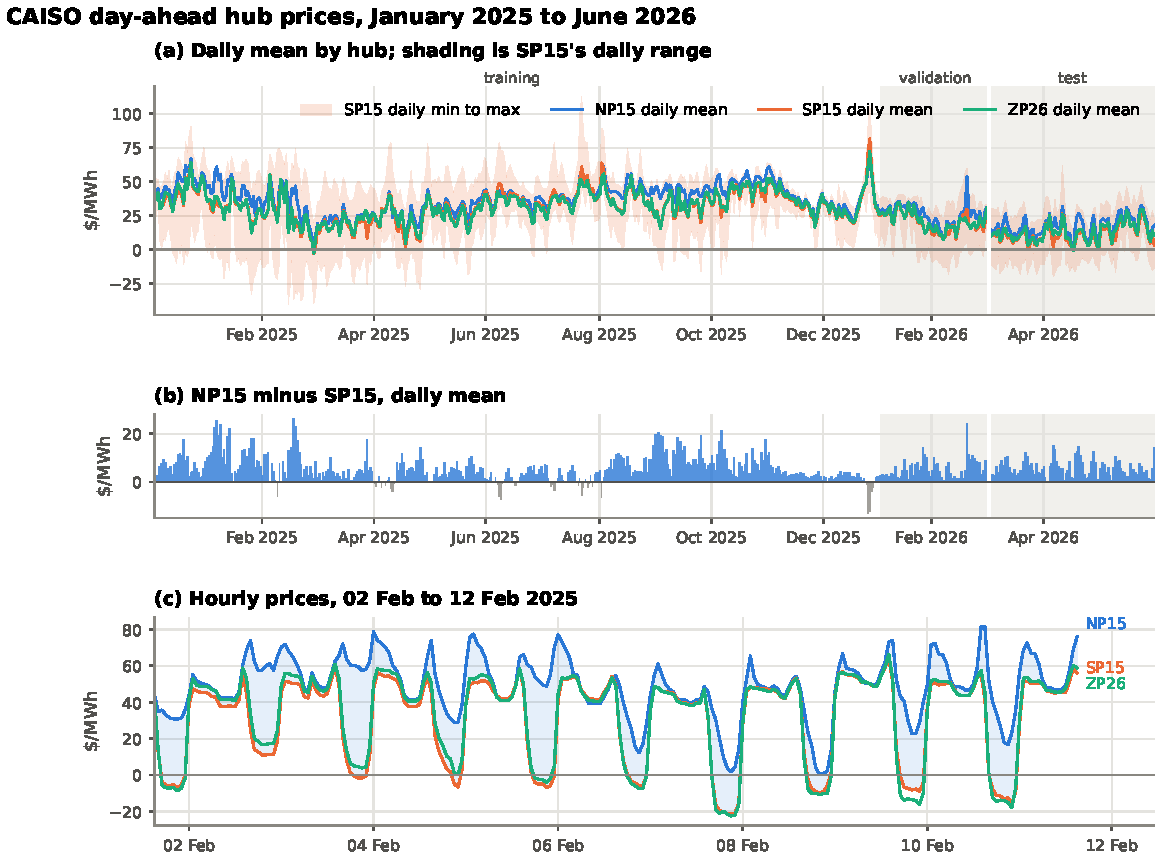
\includegraphics[width=0.86\textwidth]{figures/hub_prices.pdf}
\caption{(a)~Daily mean day-ahead price at each hub over the eighteen months, with SP15's daily range; shading marks the validation and test splits. (b)~Daily mean NP15$-$SP15 spread. (c)~The ten-day window with the widest NP15/SP15 split (February 2025): NP15 decouples for days at a time while all three hubs keep the duck-curve shape and negative midday prices.}
\label{fig:data}
\end{figure}

\subsection{Model}
Prices are standardized per hub by train-split moments. The state is
augmented with slow exponential moving averages, a per-hub level $E_t$ and
a scalar realized-movement average $v_t$, with $\alpha = e^{-1/168}$:
\begin{equation}
E_{t+1} = \alpha E_t + (1-\alpha) X_{t+1}, \qquad
v_{t+1} = \alpha v_t + (1-\alpha)\,\tfrac13 \textstyle\sum_j
\big|X_{j,t+1} - X_{j,t}\big| .
\label{eq:ema}
\end{equation}
Both are functions of the price path, so the augmented system
$(X, E, v)$ stays Markov and self-contained under simulation, requiring no
exogenous future input. The
observable $X_t \in \mathbb{R}^3$ follows
\begin{equation}
dX_t = \Big[K_\theta(z_t)\odot\big(E_t + a_\theta(c(t)) - X_t\big) +
\rho_\theta(z_t)\Big]dt
+ \mathrm{diag}\big(d_\theta(z_t)\big)\,L_\rho\, dW_t + dJ_t,
\label{eq:sde}
\end{equation}
where $c(t)$ holds three hour-of-day harmonics (a duck curve is far from
sinusoidal) plus day-of-week and day-of-year encodings; the network input
$z_t = (X_t - E_t,\; X_{1,t}-X_{2,t},\; X_{1,t}-X_{3,t},\; v_t,\; c(t))$
contains the spreads, the congestion observable of Section~\ref{sec:grid}, and is
deliberately level-free; $K_\theta \in [0.02, 2]$ per hour and
$\rho_\theta \in [-0.5, 0.5]$ are small tanh MLPs; $L_\rho$ is a learned
constant correlation factor; and $J_t$ is a compound Poisson process
with two-harmonic diurnal intensity
$\lambda(\tau) \le 0.15/$h and a
two-component (up/down) Gaussian mixture of jump vectors, shared across
hubs because spikes are system events. The model has about 13{,}000
parameters, against 9{,}504 training hours.

Training is two-stage. Stage~A
maximizes the exact likelihood of the Euler-discretized jump-diffusion.
With at most one jump per hour ($P(\ge 2) \le 1.1\%$), the one-step
transition density is a three-component Gaussian mixture,
\begin{equation}
p(x'|x) = (1{-}\lambda\Delta)\,
\mathcal{N}\big(x{+}\mu_\theta\Delta,\; \Sigma_\theta\Delta\big)
+ \lambda\Delta\!\sum_{k \in \{+, -\}} w_k
\mathcal{N}\big(x{+}\mu_\theta\Delta{+}m_k,\;
\Sigma_\theta\Delta{+}\mathrm{diag}(s_k^2)\big),
\label{eq:nll}
\end{equation}
A centering
penalty pins the batch-mean total drift, diffusion part plus
jump compensator $\lambda \bar m_J$, at zero: a bias of $0.05\sigma$/h
costs only about 0.008 nats per transition, too little for the likelihood
to notice, but compounds to a full $\sigma$ within two weeks through the
EMA. Stage~B fine-tunes
by simulated method of moments \cite{duffie1993} through
\texttt{torchsde}'s adjoint \cite{li2020}:
72-hour windows are simulated with a jump-adapted scheme (the diffusion
integrated continuously within each hour, jumps applied as discrete
updates between solver calls, since a discontinuity inside an adaptive
solver corrupts both stepping and the adjoint), and window moments are
matched to real windows: means, dispersions, increment kurtosis, spike and
negative-price frequencies, spread dispersions, and autocorrelations at
lags 1--24~h. A checkpoint is accepted only if held-out
transition likelihood stays within 0.35 nats of the Stage-A optimum; the
final model spends 0.31.

\subsection{Validation}
The model's downstream role is conditional simulation over hours-to-days,
re-anchored at observed states, so the validation protocol simulates four
non-overlapping 14-day ensembles (50 paths each) across the held-out
validation window, each initialized at the real state and real trailing
EMAs. The moment, spike-rate and half-life thresholds were fixed before
any results were seen. On the reported draw those checks all pass (Table~\ref{tab:sdeval}), though
Section~\ref{sec:seedrobust} shows that verdict is itself seed-dependent; Figures~\ref{fig:qq} and \ref{fig:paths} show
the distributional and visual comparisons. The residual mismatches inside
those passing thresholds are sizeable: simulated means sit \$3.6--5.4 high
(offsets 0.25--0.35 of a standard deviation against a 0.5 threshold),
dispersion runs 6--21\% high,
negative-price frequency reaches only $0.6$--$0.8\times$ the realized
rate, and half-lives run fast. A 59-day single-anchor free run drifts to
\$39--40 against a realized \$20--26, so the model level behaves like a
martingale only over weeks. That suffices for a daily-re-anchored controller
but rules out multi-month unconditional forecasting.

\subsubsection{Testing the marginal distribution}
The shape of
the marginal, as opposed to its moments, is tested with a
Kolmogorov--Smirnov statistic \cite{massey1951}, which measures the
largest vertical gap $D$ between two cumulative distribution functions. A
naive two-sample KS returns
$p \sim 10^{-61}$, but that test is invalid here: it assumes i.i.d. draws,
while these series are strongly autocorrelated, with an integrated
autocorrelation time implying an effective sample size of 114--193 against
a nominal 1{,}344. The valid construction is a moving-block bootstrap
\cite{kunsch1989}, which resamples contiguous blocks (length 13--72\,h,
set from the autocorrelation time) so that each resampled series keeps the
serial dependence that i.i.d. resampling would destroy, and uses those
draws to build the null distribution of $D$. That
corrected test gives
\begin{equation}
D = 0.221\text{--}0.230, \qquad p_{\text{block}} = 0.0005\text{--}0.002,
\label{eq:ks}
\end{equation}
stable across block lengths from 6 to 96\,h. The corrected $p$ is many
orders of magnitude larger than the naive one and still rejects at any
conventional level. Removing the hour-of-day profile from both series
first makes the discrepancy larger ($D = 0.225$--$0.286$,
$p = 0.0015$--$0.004$), so the mismatch is in the marginal's shape, not
in diurnal phase. A maximum CDF gap near 23 percentage points is
economically as well as statistically material.

\subsubsection{Rank histograms}
The KS test says the simulated and real marginals differ, but not how. The
rank histogram, or probability integral transform
\cite{hamill2001,gneiting2007}, says whether a forecast ensemble is biased,
too wide or too narrow.

Rank each observation $y_t$ among the
$M = 50$ ensemble members drawn for that same hour,
$R_t = \#\{i : s^{(i)}_t < y_t\}$. If observation and members are draws
from the same predictive distribution they are exchangeable, so $R_t$ is
uniform on $\{0,\dots,M\}$ however wide that distribution is, which
removes width as a confound, and the histogram's shape diagnoses the
error: a slope means bias, a dome over-dispersion, a U under-dispersion.
Ranks inherit the price autocorrelation, so significance comes from a
moving-block bootstrap of the rank series (block 54--74\,h from its
integrated autocorrelation time).

\begin{equation}
\overline{\mathrm{PIT}} = \bar{R}/M
= 0.347,\; 0.310,\; 0.335 \quad\text{vs } 0.5 \text{ calibrated},
\label{eq:pit}
\end{equation}
with bootstrap 95\% intervals $[0.250, 0.452]$, $[0.229, 0.405]$,
$[0.265, 0.408]$ for NP15/SP15/ZP26; none contains $0.5$.
Observations fall below the entire ensemble 2.8/1.9/2.0 times more
often than the $1/51$ expected, and above it only 0.9/0.3/0.3 times as
often. Figure~\ref{fig:calibration} shows histograms sloping steeply
downward on every hub.

Calibration is rejected, and the main error is in the level: real
prices land in the bottom third of the simulated distribution. Measured within paths, the
like-for-like comparison, simulated standard deviation is
1.04--1.14$\times$ realized, against the 1.07--1.21 obtained by pooling
across the ensemble. Dispersion diagnostics disagree (the
within-path ratio suggests mild over-dispersion, the quadratic rank
contrast the opposite), so no direction is claimed for width. The level
bias can be measured directly: within each
re-anchored window the SP15 ensemble mean starts \$3.4 above realized on
day 0, immediately after anchoring at the true state, and drifts a
further $+\$3.0$ by day 13, while the realized path fell \$3.3. Only the
$+\$3.0$ is model error; the realized decline continued a trend the model
had no information about.

\begin{figure}[tbp]
\centering
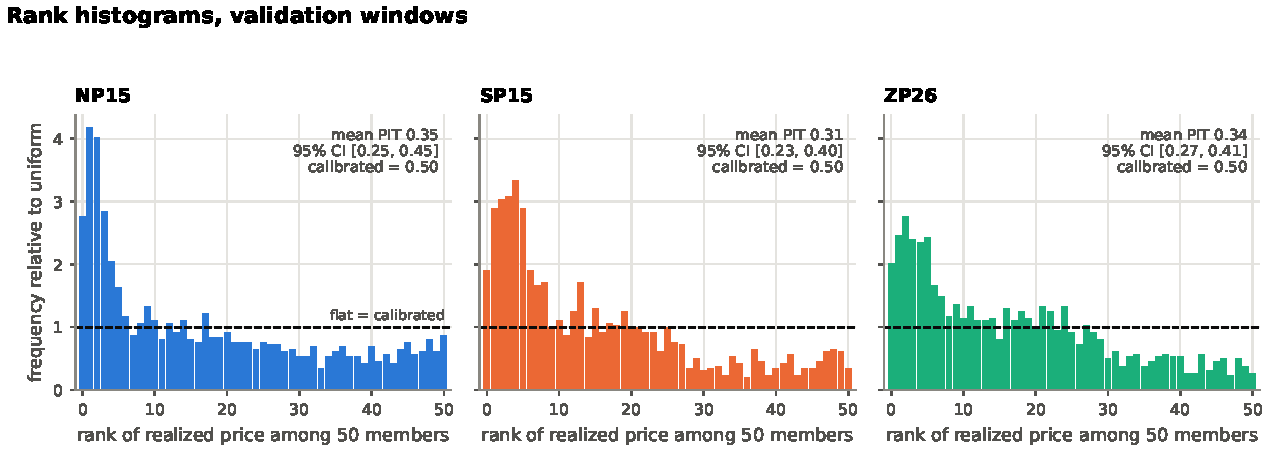
\includegraphics[width=\textwidth]{figures/rank_histograms.pdf}
\caption{Rank of each realized hourly price among the 50 ensemble members simulated for that hour, over the four validation windows. Mean PIT and its block-bootstrap 95\% interval are printed in each panel.}
\label{fig:calibration}
\end{figure}

\subsection{Sensitivity to the simulation seed}
\label{sec:seedrobust}

The validation protocol was rerun over 200 independent seeds
(Figure~\ref{fig:seedrobust}): 12 of the 15 checks
pass on every seed, but the half-life criterion passes in only
87.5\% of draws on NP15 and 79.0\% on SP15 (ZP26 always passes). Across
seeds the half-life ratio averages 0.538 and 0.535 on those two hubs
against a 0.5 floor, dipping to 0.442 and 0.458 at worst. Across all draws, 73.5\% of
seeds reproduce 15/15; 19.5\% give 14/15 and 7.0\% give 13/15.

\begin{figure}[tbp]
\centering
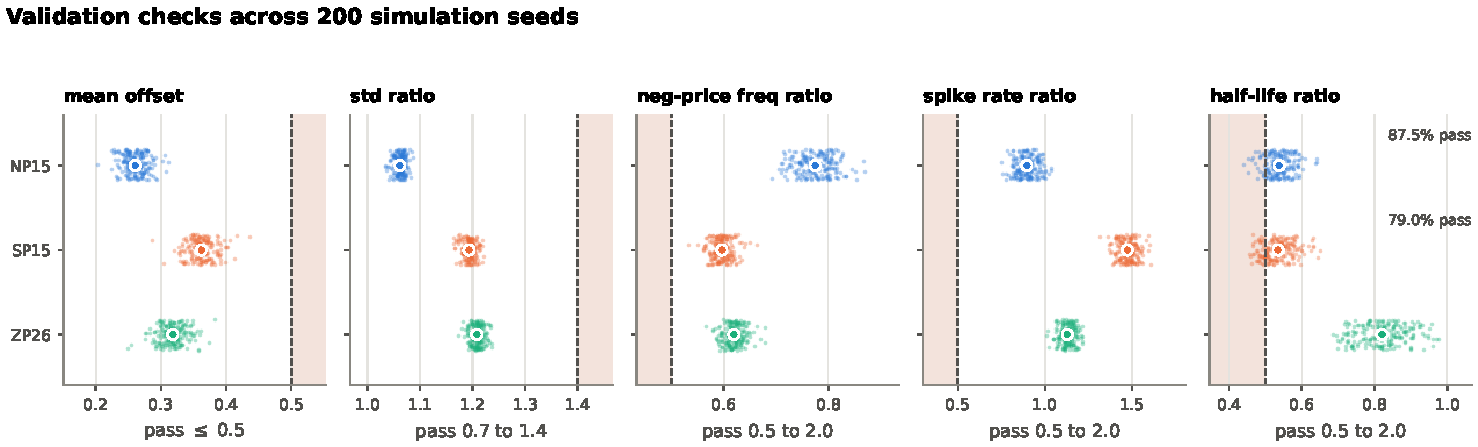
\includegraphics[width=0.92\textwidth]{figures/seed_robustness.pdf}
\caption{Each criterion across 200 seeds against its threshold. The
half-life criterion on NP15 and SP15 straddles its floor; every other
check clears with margin on every draw.}
\label{fig:seedrobust}
\end{figure}

\subsubsection{A seasonal-OU baseline}
A seasonal-mean
Ornstein--Uhlenbeck process \cite{uhlenbeck1930}, the standard
mean-reverting benchmark for power prices \cite{lucia2002}, fitted by
exact Gaussian MLE on the same
split with the same Fourier clock basis and the same jump specification,
is the parametric control.
Across three variants: plain OU reaches held-out one-step NLL $-0.95$ and
8 of the 15 moment-and-rate checks; adding jumps gives $-2.23$ and 7/15;
adding the same EMA level anchor gives $-2.22$ and 12/15; the neural SDE
reaches $-2.88$ and 15/15. The neural model is ahead of these three
variants on held-out likelihood and on spike frequency, which plain OU
barely produces (ratio 0.00--0.16). But the EMA-anchored OU closes most of
the gap with a small fraction of the parameters, and holds its level
better over a 59-day free run at NP15 (simulated mean \$26.8 against a
realized \$25.8, versus \$41.0 for the neural model). Every variant, parametric and neural, fails the
block-bootstrap KS test of \eqref{eq:ks}, locating the failure at the
level of the Gaussian-increment jump-diffusion model class.

\begin{table}[tbp]
\centering\small
\begin{tabular}{lrrrrrr}
\toprule
 & \multicolumn{2}{c}{mean (\$/MWh)} & \multicolumn{2}{c}{std (\$/MWh)}
 & \multicolumn{2}{c}{negative hours (\%)}\\
hub & real & sim & real & sim & real & sim\\
\midrule
NP15 & 25.8 & 29.4 & 14.4 & 15.3 & 5.9 & 4.6\\
SP15 & 20.3 & 25.7 & 15.5 & 18.4 & 17.6 & 10.5\\
ZP26 & 20.9 & 25.7 & 15.5 & 18.7 & 18.1 & 11.3\\
\midrule
 & \multicolumn{2}{c}{spikes / 1000 h} & \multicolumn{2}{c}{half-life (h)}
 & \multicolumn{2}{c}{KS $D$ (median)}\\
 & real & sim & real & sim & \multicolumn{2}{c}{}\\
\midrule
NP15 & 5.2 & 5.1 & 8.7 & 5.0 & \multicolumn{2}{c}{0.275}\\
SP15 & 11.9 & 17.2 & 8.2 & 4.9 & \multicolumn{2}{c}{0.259}\\
ZP26 & 15.7 & 17.6 & 5.3 & 4.8 & \multicolumn{2}{c}{0.263}\\
\bottomrule
\end{tabular}
\caption{Validation criteria over re-anchored 14-day ensembles. Spike
$=$ hourly move exceeding \$25/MWh; half-life from AR(1) fits to
hour-of-day-deseasonalized residuals. All fifteen moment-and-rate checks
(mean offset $\le 0.5\sigma$; std ratio in $[0.7, 1.4]$; negative-rate,
spike-rate and half-life ratios in $[0.5, 2]$) pass. The KS column is the
median per-window statistic; the block-bootstrap test of \eqref{eq:ks}
rejects equal marginals on every hub ($p \approx 0.001$).}
\label{tab:sdeval}
\end{table}

\begin{figure}[tbp]
\centering
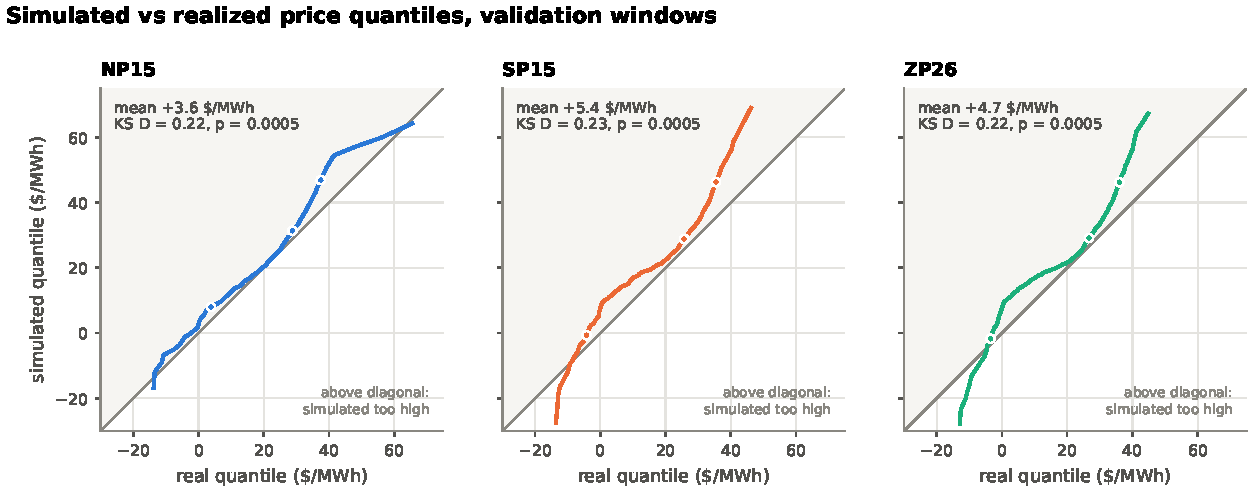
\includegraphics[width=0.92\textwidth]{figures/marginal_qq.pdf}
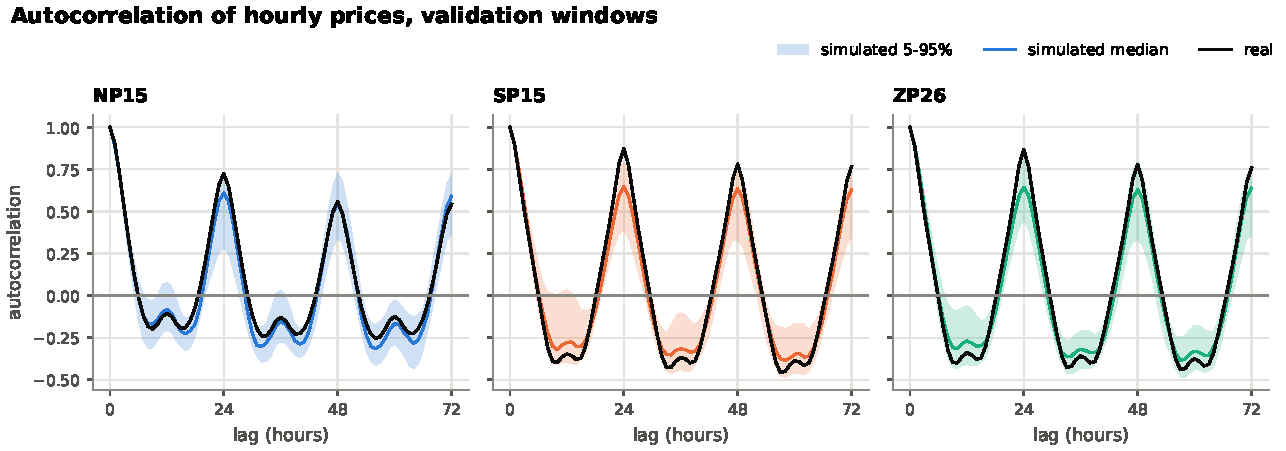
\includegraphics[width=0.92\textwidth]{figures/autocorrelation.pdf}
\caption{Top: quantiles of simulated against real prices over the validation windows, with the mean offset and block-bootstrap KS result for each hub. Bottom: autocorrelation to lag 72~h. The simulated median tracks the real curve's shape, but on SP15 and ZP26 the real daily peaks sit at or above the top of the simulated 5--95\% band.}
\label{fig:qq}
\end{figure}

\begin{figure}[tbp]
\centering
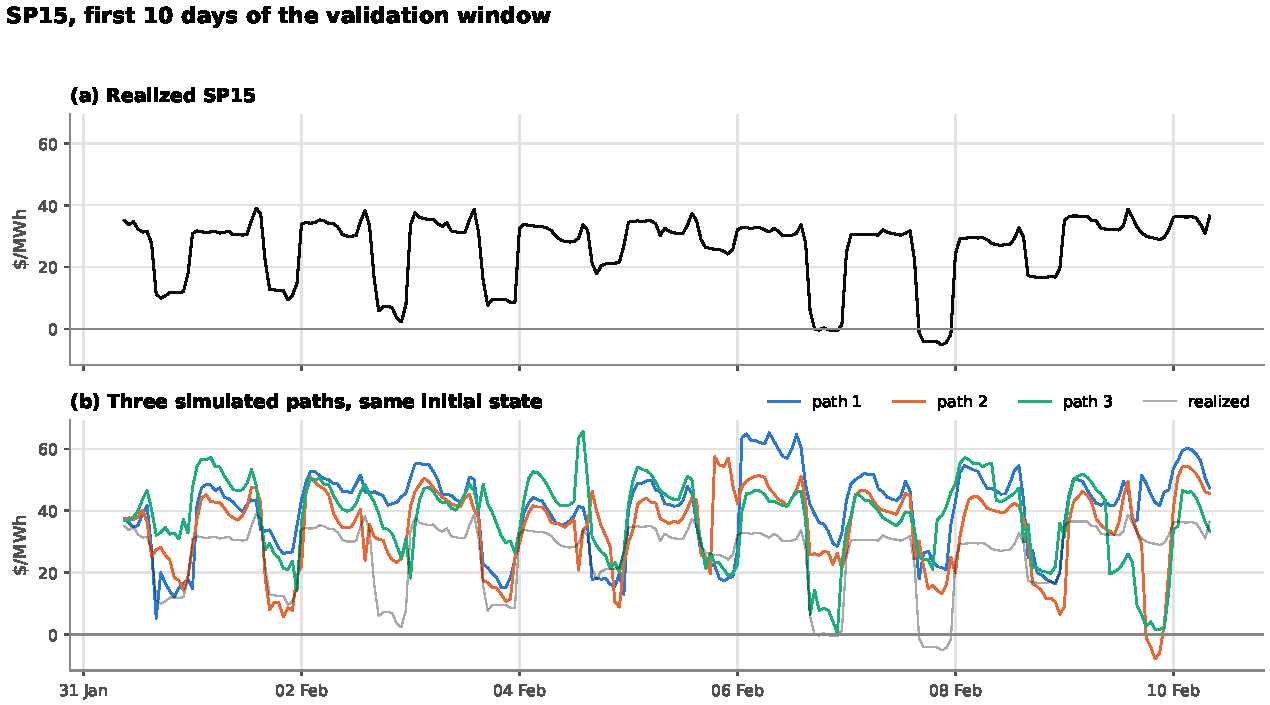
\includegraphics[width=0.80\textwidth]{figures/simulated_paths.pdf}
\caption{Real SP15 over the first ten validation days (top) and three simulated paths from the same initial state, with the realized path in grey for reference (bottom). The simulated days have the diurnal valleys and occasional negative dips but sit higher and lack the flat-top, sharp-plunge profile of the real ones.}
\label{fig:paths}
\end{figure}

\section{Stochastic control}
\label{sec:control}

Dispatching a battery under uncertainty is a stochastic control problem.
At each hour the operator picks a power level without knowing future
prices, and the right choice turns on what the stored energy will be worth
later. That is captured by the value function: the best
expected revenue achievable from now to the end of the horizon, given the
current state of charge and the current prices. Dynamic programming
characterizes it through the Hamilton--Jacobi--Bellman (HJB) equation,
which propagates value backwards from the end of the day. The HJB
is restated as a backward stochastic differential equation
\cite{pardoux1990} and solved with neural networks
\cite{weinan2017,han2018}, a method whose cost grows linearly rather than
exponentially with the number of price nodes. At the three hubs used here
a grid solution is still affordable, and it is the benchmark.

A price-taking battery at SP15: 25~MW / 100~MWh, one-way efficiency
$\sqrt{0.88}$, \$2/MWh throughput degradation cost, dispatched over daily
horizons with terminal salvage $\pi \approx \$36.5$/MWh (efficiency-%
discounted median overnight price) and day-chained SOC. Control $u \in [-\bar P, \bar P]$ is power to the grid, so state of charge
and running reward evolve as
\begin{equation}
dS_t = \varphi(u_t)\,dt, \quad
\varphi(u) = \begin{cases} -u/\eta_d & u \ge 0 \\ -\eta_c u & u < 0
\end{cases}, \qquad r(P, u) = Pu - c_{\deg}|u| ,
\label{eq:soc}
\end{equation}
so discharging drains more SOC than it delivers and charging stores less
than it draws. The value function is
\begin{equation}
V(t, s, x) = \sup_{u_\cdot}\ \mathbb{E}\left[\int_t^T
r\big(P(X_{t'}), u_{t'}\big)\,dt' + g(S_T)\ \middle|\
S_t = s,\ X_t = x\right],
\label{eq:value}
\end{equation}
where $g(S_T) = \pi\,\mathrm{clip}(S_T, 0, C)$ is the terminal salvage and
the supremum runs over admissible controls. Dynamic programming turns
\eqref{eq:value} into the HJB equation
\begin{equation}
\partial_t V + \mu_\theta^\top \nabla_x V + \tfrac12
\mathrm{Tr}\big(\Sigma_\theta \nabla^2_x V\big)
+ \lambda\,\mathbb{E}_Z\big[V(x{+}Z) - V(x)\big]
+ \max_{u \in U(s)}\big[r(P(x),u) + \varphi(u)\,\partial_s V\big] = 0,
\label{eq:hjb}
\end{equation}
a partial integro-differential equation because of the jump term.
Two approximations make it tractable. First, Taylor-expanding $V$ in the jump size,
$\mathbb{E}_Z[V(x{+}Z) - V(x)] = \bar m_J^\top \nabla_x V +
\tfrac12 \mathrm{Tr}(M_2 \nabla_x^2 V) + O(\mathbb{E}|Z|^3)$, and
absorbing the first two moments into the coefficients gives the
moment-matched generator
\begin{equation}
\tilde\mu_{\text{eff}} = \mu_\theta + \lambda\,\bar m_{\text{jump}}, \qquad
\tilde\Sigma_{\text{eff}} = \Sigma_\theta + \lambda\,M_{2,\text{jump}}, \qquad
M_{2,\text{jump}} = \mathbb{E}[ZZ^\top] ,
\label{eq:momentmatch}
\end{equation}
which turns the PIDE into a PDE. The cost of that step was measured: the
reduced-problem DP solved with exact jump transitions against
moment-matched ones differs by 0.2\% median and 1.7\% max. Second, the
noiseless SOC direction is viscosity-regularized with artificial noise
$\varepsilon_{\text{soc}}\,dW^0$ \cite{crandall1992}. The deep BSDE
scheme reads gradients off diffusion loadings and would otherwise be blind
to $\partial_s V$, the one quantity the control depends on. The
Hamiltonian collects every term involving the control,
\begin{equation}
H(x, s, q) = \max_{u \in U(s)} \big[\, r(P(x), u) + \varphi(u)\,q \,\big],
\qquad
U(s) = \Big[-\min\big(\bar P, \tfrac{(C-s)^+}{\eta_c \Delta}\big),\;
\min\big(\bar P, \tfrac{\eta_d s^+}{\Delta}\big)\Big],
\label{eq:hamiltonian}
\end{equation}
with $U(s)$ clamping power so the SOC bounds cannot be crossed within a
step. Since $r + \varphi q$ is piecewise linear in $u$, the maximiser is
bang-bang with interpretable thresholds: discharge at full power when
$P > q/\eta_d + c_{\deg}$, charge at full power when
$P < \eta_c q - c_{\deg}$, and otherwise idle. Here $q = \partial_s V$ is
the marginal value of stored energy, so the battery acts when the
price clears that marginal value after efficiency and degradation
frictions.

The scheme then runs on an uncontrolled forward system in the
augmented state $\bar X = (S, X) \in \mathbb{R}^4$,
\begin{equation}
d\bar X_t = \begin{pmatrix} 0 \\ \tilde\mu_{\text{eff}} \end{pmatrix} dt
+ \bar\sigma \, d\bar W_t, \qquad
\bar\sigma = \begin{pmatrix} \varepsilon_{\text{soc}} & 0 \\
0 & \tilde\Sigma_{\text{eff}}^{1/2} \end{pmatrix},
\label{eq:forward}
\end{equation}
whose first noise channel is the artificial SOC diffusion. Defining
$Y_t = V(t,\bar X_t)$ and $Z_t = \bar\sigma^\top \nabla_{\bar X} V$, so
that $Z^{(\text{soc})} = \varepsilon_{\text{soc}}\,\partial_s V$, It\^o's formula plus the PDE
cancel every second-order term and leave the backward SDE
\begin{equation}
dY_t = -\,H\big(X_t, S_t, Z^{(\text{soc})}_t/\varepsilon_{\text{soc}}\big)\,dt
+ Z_t^\top d\bar W_t, \qquad Y_T = \pi S_T,
\label{eq:bsde}
\end{equation}
whose (unique, Lipschitz-driver) solution is the value function:
the marginal value is read off the SOC-noise loading as
$q = Z^{(\text{soc})}/\varepsilon_{\text{soc}}$. The deep BSDE scheme parameterizes $Y_0$ and each hourly $Z_{t_k}$ with a
small MLP (conditioned on the frozen day instance: EMAs, calendar) and
discretizes \eqref{eq:bsde} on the hourly grid $t_k = k$,
\begin{equation}
Y_{k+1} = Y_k - H\big(X_k, S_k, Z^{(\text{soc})}_k/\varepsilon_{\text{soc}}\big)\Delta
+ Z_k^\top \Delta\bar W_k, \qquad
\min_\xi\ \mathbb{E}\big[(Y_{24} - g(S_{24}))^2\big],
\label{eq:deepbsde}
\end{equation}
rolling forward over sampled training days with $S_0 \sim U[0, C]$ and
training all networks jointly on the terminal-matching loss. Uniqueness of
the Lipschitz-driver BSDE solution \cite{pardoux1990} is what ties the
scheme to the PDE, and convergence of this class of solver is studied in
\cite{hanlong2020}: any
$(Y, Z)$ satisfying \eqref{eq:deepbsde} and the terminal condition
is the value function and its gradient along the forward paths, and
the optimal control is recovered pointwise as the argmax in
\eqref{eq:hamiltonian}.

At this problem size, dynamic programming on a grid is also feasible. The
state is $(S, X) \in \mathbb{R}^4$ plus time, and each day instance has
its own frozen regime states and calendar, so the grid is re-solved every
day. With 21 SOC nodes and 29 nodes per hub the grid has
$21 \times 29^3 \approx 5.1\times10^5$ nodes per hour. The price
transition cannot be applied densely ($29^6 \approx 6\times10^8$ entries)
or as a per-dimension sweep, because the fitted covariance is
state-dependent and correlated across hubs. But the one-hour conditional
spread is a few tenths of a unit, so a Gaussian kernel truncated to
$\pm 5$ cells per hub keeps about $3\times10^7$ nonzeros per hour, and the
control maximization needs only interpolation in SOC. A full 24-hour
backward induction then takes about three minutes on one core. Solved for
each of the 90 test days and dispatched on realized prices with the same
information set and salvage as the deep BSDE policy, the grid DP earns
\$229{,}511 against the deep BSDE's \$229{,}885 (paired daily
$t = -0.06$, DP ahead on 52 of 90 days): at three hubs the two methods
tie. The deep BSDE's advantage lies beyond this problem. The truncated
kernel grows as $29^d \times 11^d$, reaching about $10^{10}$ nonzeros per
hour at four hubs and $3\times10^{12}$ at five, while the BSDE adds one
network output per hub and serves every day instance from a single
training run.

\subsection{Cross-check against dynamic programming}
The check solves a self-contained reduced problem
(SP15 only, other hubs perfectly coupled) with two independent
methods: backward-induction DP on a $(S, x)$ grid and the identical deep
BSDE code with a one-dimensional price state, compared at 60 state-time
points ($t \in \{0,6,12,18\}$~h $\times$ $s \in \{10,50,90\}$~MWh
$\times$ five price levels), with a pre-registered 15\% tolerance. On the spatial grid, backward dynamic programming computes
\begin{equation}
V(t_k, s, x) = \max_{u \in U(s)} \left\{ r(P(x), u)\Delta + \mathbb{E}\left[V(t_{k+1}, s + \varphi(u)\Delta, X_{k+1}) \;\middle|\; X_k = x\right] \right\} ,
\label{eq:grid_dp}
\end{equation}
with expectations taken over discretized transition matrices. Any breach
of the 15\% tolerance triggers a rerun on a grid with both dimensions
doubled.

The final
configuration, with $\varepsilon$ annealed $8 \to 2.5$~MWh/$\sqrt{\text{h}}$
during training, a linear terminal extension and horizon-scaled
$\varepsilon$ for the sub-horizon solves, brings 57 of 60 points inside
tolerance, with a worst residual of 32.2\% (Figure~\ref{fig:dpcheck});
Section~\ref{sec:analysis} discusses the three points outside it. The
configuration used for dispatch, the full 24-hour solve, passes at all 15 of its points (median 5.4\%, max
8.9\%). The training loss and policy non-degeneracy checks are in
Figure~\ref{fig:bsdeloss}: across sampled day instances the learned policy
charges in 7.6\% of hours, discharges in 16.9\%, idles in 75.5\%, and
swings 66 of the 100~MWh SOC range.

\begin{figure}[tbp]
\centering
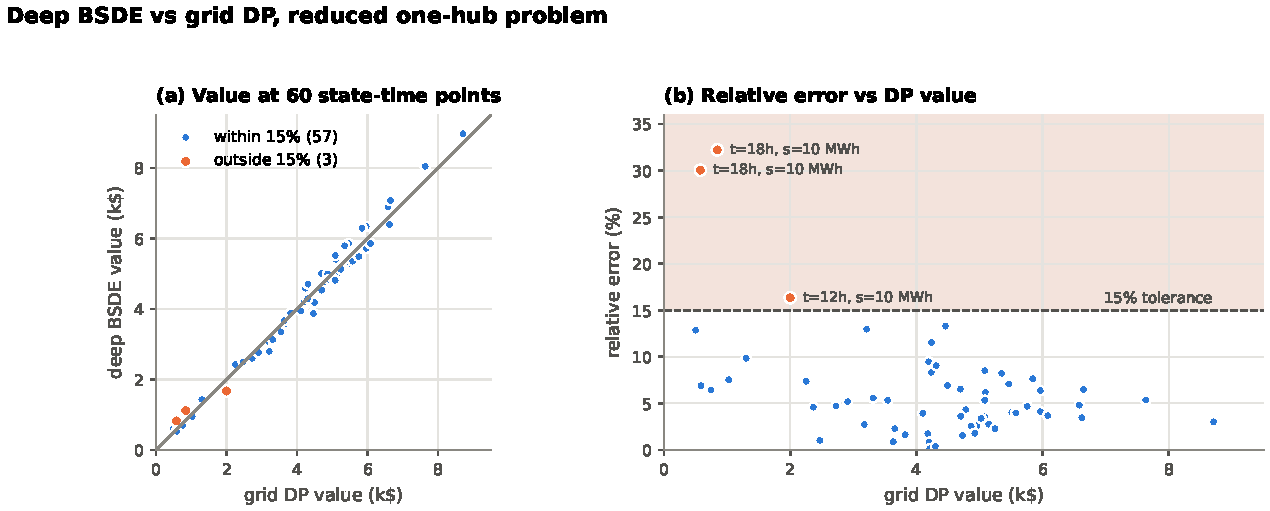
\includegraphics[width=0.90\textwidth]{figures/dp_cross_check.pdf}
\caption{Reduced-problem cross-check at 60 state-time points. (a)~Deep BSDE value against grid DP. (b)~Relative error against the DP value: the three points outside the 15\% tolerance are the three smallest values, all at 10~MWh with 6--12 hours left.}
\label{fig:dpcheck}
\end{figure}

\begin{figure}[tbp]
\centering
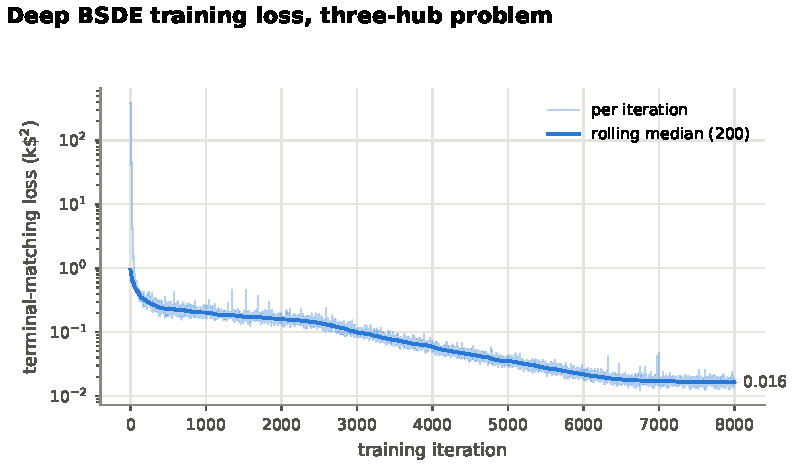
\includegraphics[width=0.46\textwidth]{figures/bsde_loss.pdf}
\caption{Deep BSDE terminal-matching loss on the full three-hub problem.}
\label{fig:bsdeloss}
\end{figure}

\section{Implementation}

Everything is Python. Prices come from CAISO OASIS through
\texttt{gridstatus} (18 monthly requests, cached locally); the grid layer
uses \texttt{pandapower}/\texttt{pypower} \cite{thurner2018} for the case
data and PTDFs and \texttt{scipy}'s HiGHS \cite{huangfu2018} for the
DC-OPF and its duals. The price model is written in \texttt{torch}, with
\texttt{torchsde} \cite{li2020} handling the Stage~B rollouts and their
adjoint, the EMA states carried inside the solver state. The deep BSDE
solver is custom, with one network per time step, and the same code
serves the full and the reduced control problems. The full-state grid DP
benchmark applies a sparse truncated-Gaussian transition kernel with
\texttt{scipy.sparse}, and the perfect-foresight LP is solved with
\texttt{cvxpy} \cite{diamond2016}.

Baselines: (i) threshold rules that charge below the 25th and discharge
above the 75th percentile, with static (train-period) or rolling
(trailing-168~h) percentiles; (ii) an hour-of-day schedule that charges in
the five cheapest and discharges in the four dearest hours of the training
split's mean diurnal profile, five and four being the full-power hours
needed to fill and to drain the battery; (iii) the grid DP policy on the
full four-dimensional state (Section~\ref{sec:control}); and (iv) the
perfect-foresight LP over the whole test horizon,
\begin{equation}
\begin{aligned}
\max_{u_{\text{ch}}, u_{\text{dis}}}\; &\sum_{t=1}^T \Big( P_t u_{t,\text{dis}} - P_t u_{t,\text{ch}} - c_{\text{deg}}(u_{t,\text{dis}} + u_{t,\text{ch}}) \Big)\Delta + g(S_T) \\
\text{s.t.}\;& S_{t+1} = S_t - \frac{u_{t,\text{dis}}}{\eta_d}\Delta + \eta_c u_{t,\text{ch}}\Delta,\quad 0 \le S_t \le C,
\end{aligned}
\label{eq:pf_lp}
\end{equation}
an upper bound under perfect price foresight.

\section{Results}
\label{sec:results}

The policy was dispatched on realized SP15 prices over the untouched test
quarter (April--June 2026, 2{,}160 hours, 90 day-chained instances) and,
separately, on simulated price paths. Table~\ref{tab:backtest} and
Figure~\ref{fig:backtest} give the comparison.

\begin{table}[tbp]
\centering\small
\begin{tabular}{lrrrrrr}
\toprule
 & \multicolumn{5}{c}{realized revenue (\$)} & \\
\cmidrule(lr){2-6}
window & deep BSDE & grid DP & hour-of-day & naive rolling & naive static
& \% of PF\\
\midrule
April & 81{,}293 & 82{,}359 & 77{,}823 & 45{,}795 & $-42$ & 90.9\\
May & 81{,}628 & 82{,}014 & 80{,}589 & 29{,}959 & 3{,}550 & 87.3\\
June & 66{,}965 & 65{,}139 & 68{,}758 & 22{,}714 & 1{,}214 & 87.2\\
\midrule
total & 229{,}885 & 229{,}511 & 227{,}170 & 98{,}468 & 4{,}722 &
88.5\\
\bottomrule
\end{tabular}
\caption{Battery revenue on realized test prices, 25~MW / 100~MWh at SP15.
Perfect-foresight totals are 89{,}397 / 93{,}482 / 76{,}825 / 259{,}704.
The last column is the deep BSDE policy as a fraction of the
perfect-foresight ceiling; grid DP is the full-state benchmark of
Section~\ref{sec:control}.}
\label{tab:backtest}
\end{table}

The deep BSDE policy earns \$229{,}885 over the quarter, 88.5\% of the
perfect-foresight ceiling of \$259{,}704. Each capture rate carries a
moving-block bootstrap confidence interval (5-day blocks, 20{,}000
resamples, ratio of sums within each resample): the policy captures
88.5\% (95\% CI 84.8--92.6), the hour-of-day rule 87.5\% (83.4--92.0),
the rolling percentile rule 37.9\% (27.6--47.8), and the static rule
1.8\% ($-0.3$ to 5.1).

The static threshold rule, charging below the train-period 25th
percentile and discharging above the 75th, earns almost nothing
(\$4{,}722) because the train-to-test regime shift moved prices out from
under its fixed thresholds: only 6 of 2{,}160 test hours clear its
\$46/MWh discharge trigger. The rolling variant, which re-estimates its
percentiles over a trailing week, recovers to \$98{,}468. The hour-of-day
rule charges in the five cheapest hours of the training split's mean
diurnal profile (10:00--14:59) and discharges in the four dearest
(18:00--21:59); five and four are the full-power hours it takes to fill
an empty battery, $C/(\eta_c \bar P) = 4.3$, and to drain a full one,
$\eta_d C/\bar P = 3.8$. Chosen once and never updated, it earns
\$227{,}170.

Against that rule the stochastic policy is ahead by 1.0 percentage point
of the ceiling (\$30/day). The moving-block 95\% CI of $-2.6$ to $+4.5$
points includes zero at every block length tested from 1 to 10 days, the
paired daily $t$ is 0.45, the policy is ahead on 51 of 90 days, and the
rule wins June outright. The two trade almost the same volume (18{,}131
against 17{,}983~MWh). In this market a fixed diurnal schedule captures
nearly all of what the stochastic controller earns. The grid DP policy of Section~\ref{sec:control},
solving the same control problem without neural networks, earns
\$229{,}511 (88.4\%), level with the deep BSDE.

The policy charges through the midday trough, but 83.7\% of its discharge falls
between midnight and 07:00 and only 13.6\% between 18:00 and 22:00, and it
ends the average day holding 86.6~MWh (Figure~\ref{fig:dispatch}). The
terminal salvage causes this: late in the day $q$ approaches
$\pi = \$36.5$/MWh, which puts the discharge threshold at
$\pi/\eta_d + c_{\deg} \approx \$41$, well above test-quarter evening
prices (mean \$25), so the policy carries its energy past midnight and
sells it once the next day's solve starts with a lower $q$. The salvage
comes from the training split's overnight median and is badly
mis-calibrated for a quarter whose SP15 mean is \$11.4.

On simulated price paths (198 draws of 28 days, re-anchored at three
real test states) the policy earns \$89{,}031 on average with a
standard deviation of \$6{,}872 across draws (ratio 13.0) and a median
maximum drawdown of \$2{,}358. The ratio is mean over standard deviation
across scenarios, not an annualized Sharpe ratio, and it describes
stability under the model's own price paths, which carry the biases of
Section~\ref{sec:sde}.

\begin{figure}[tbp]
\centering
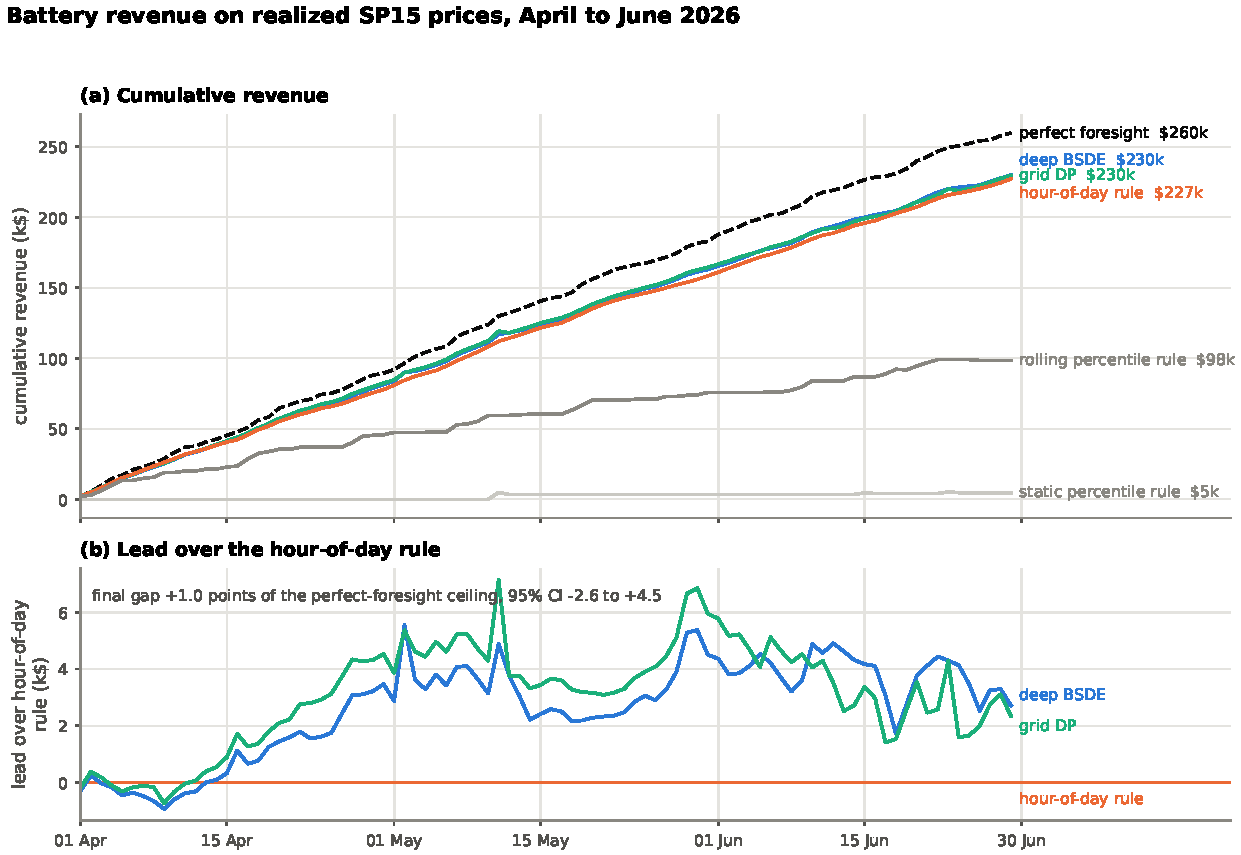
\includegraphics[width=0.88\textwidth]{figures/backtest_pnl.pdf}
\caption{(a)~Cumulative revenue on realized SP15 day-ahead prices over the April--June 2026 test quarter. (b)~Running lead of the deep BSDE and grid DP policies over the fixed hour-of-day schedule. Both build a lead of \$5--7k by May and give most of it back in June.}
\label{fig:backtest}
\end{figure}

\begin{figure}[tbp]
\centering
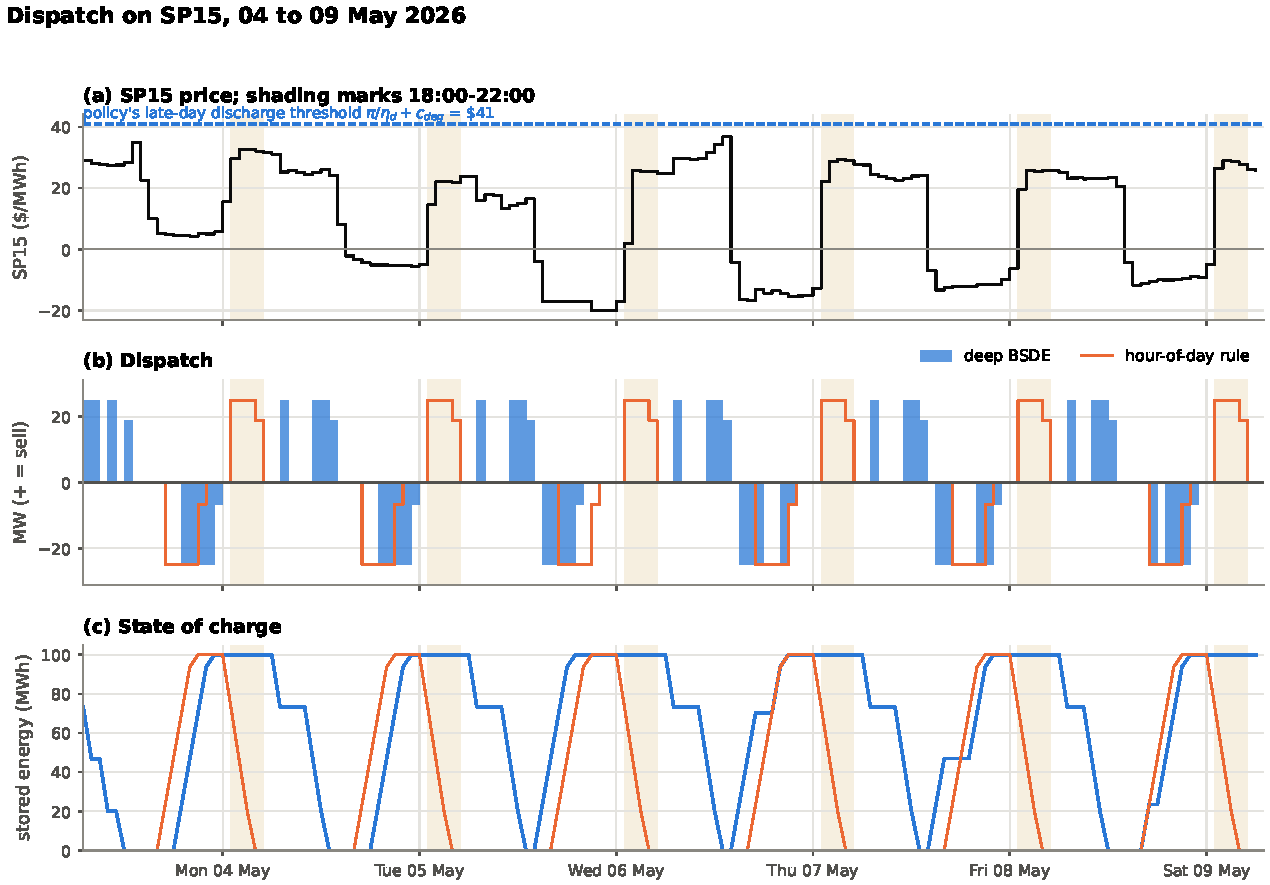
\includegraphics[width=0.78\textwidth]{figures/dispatch_detail.pdf}
\caption{Six days of dispatch in May 2026, deep BSDE policy against the hour-of-day rule. The policy fills in the negative-price midday trough, holds through the evening because its late-day discharge threshold (dashed) sits above evening prices, and sells after midnight.}
\label{fig:dispatch}
\end{figure}

\section{Discussion}
\label{sec:analysis}

\subsection{The backtest}

The policy finishes 1.0 point of the perfect-foresight ceiling ahead of
the fixed schedule, about \$30 a day, with a paired $t$ of 0.45 and a 95\%
interval of $-2.6$ to $+4.5$ points. A single quarter cannot separate an
edge that small from zero. Solar gives the 2026 CAISO day almost the same
shape every day, so a schedule read off the training year's mean day
already collects most of the spread. Grid DP on the same price model does
no better than the deep BSDE.

Three things work against the policy. The price model's half-lives
are 0.57--0.91 of the observed ones, and a model that expects dips to
close within a few hours puts too little value on holding energy through
them. It produces negative prices at 0.6--0.8 times the validation-window
rate, while SP15 cleared below zero in 34\% of test-quarter hours. The
terminal salvage, set from training-year overnight prices, sits above
test-quarter evening prices, which is why the policy sells after midnight.

The 88.5\% capture is measured on realized prices, so the model's level
bias reaches it only through the trained policy. The simulated-path
statistics in Section~\ref{sec:results} are produced by the model itself
and carry the bias in full.

\subsection{Price-model timescales}

In the data, deseasonalized system levels revert with a 13.0\,h half-life
and the two hub spreads with 4.8--5.2\,h, a spread-to-level ratio of 0.38.
The fitted SDE gives 4.1\,h for the level and 3.2--3.5\,h for the spreads,
a ratio of 0.80. Linearizing the level dynamics as $\dot L = K(E-L)$,
$\dot E = (L-E)/\tau$ with $\tau = 168$\,h shows that $K$ supplies 97\% of
the relaxation rate. A 13.0\,h half-life needs $K \approx 0.047$/h; the
fitted values are 0.15--0.17.

Four variants were trained against this, each on three to five seeds
(Table~\ref{tab:variants}, Figure~\ref{fig:twofactor}). A two-factor drift
with separate level and spread reversion rates left the level half-life
at 4.3--5.5\,h. Adding deseasonalized autocorrelations to the Stage~B
moment set reduced the standardized mean offsets from 0.25--0.35 to
0.035--0.045 and did not move the half-life. Fixing $K_{\text{level}}$ at
its empirical value of 0.0519/h raised the level half-life to 8.2--18.9\,h,
but stationary variance scales as $\sigma^2/(2\kappa)$ and grew by a
factor of 3.6. Rescaling the diffusion and jump amplitudes by
$\sqrt{\kappa_{\text{new}}/\kappa_{\text{ref}}}$ restored the variance,
and one of the three seeds then passed all fifteen moment checks with an
8.5\,h level half-life. The rank-histogram test rejected calibration for
every variant and seed on which it was run.

The next part of the model to replace is the innovation distribution,
which none of the four variants changes: every one uses Gaussian increments
and a two-component Gaussian jump mixture, and these may not have the tails
of hourly power prices.

\begin{table}[tbp]
\centering\small
\begin{tabular}{lcccc c}
\toprule
variant & seeds & level half-life (h) & spread/level & held-out NLL
& moment checks\\
\midrule
incumbent & 1 & 4.1 & 0.80 & $-2.88$ & 15\\
two-factor drift & 5 & 4.3--5.5 & 0.78--0.95 & $-3.03$ to $-2.89$ & 14 (1 seed)\\
ACF moments in Stage~B & 5 & 4.0--4.5 & 0.71--0.80 & $-3.04$ to $-2.87$ & 14--15\\
pinned reversion rates & 3 & 8.2--18.9 & 0.31--0.56 & $-3.06$ to $-2.81$ & 5--13\\
pinned, noise rescaled & 3 & 5.0--8.5 & 0.51--1.03 & $-3.08$ to $-2.84$ & 11--15\\
\midrule
observed & & 13.0 & 0.38 & & \\
\bottomrule
\end{tabular}
\caption{Price-model variants, ranges across training seeds. Moment checks
are out of 15, as in Table~\ref{tab:sdeval}.}
\label{tab:variants}
\end{table}

\begin{figure}[tbp]
\centering
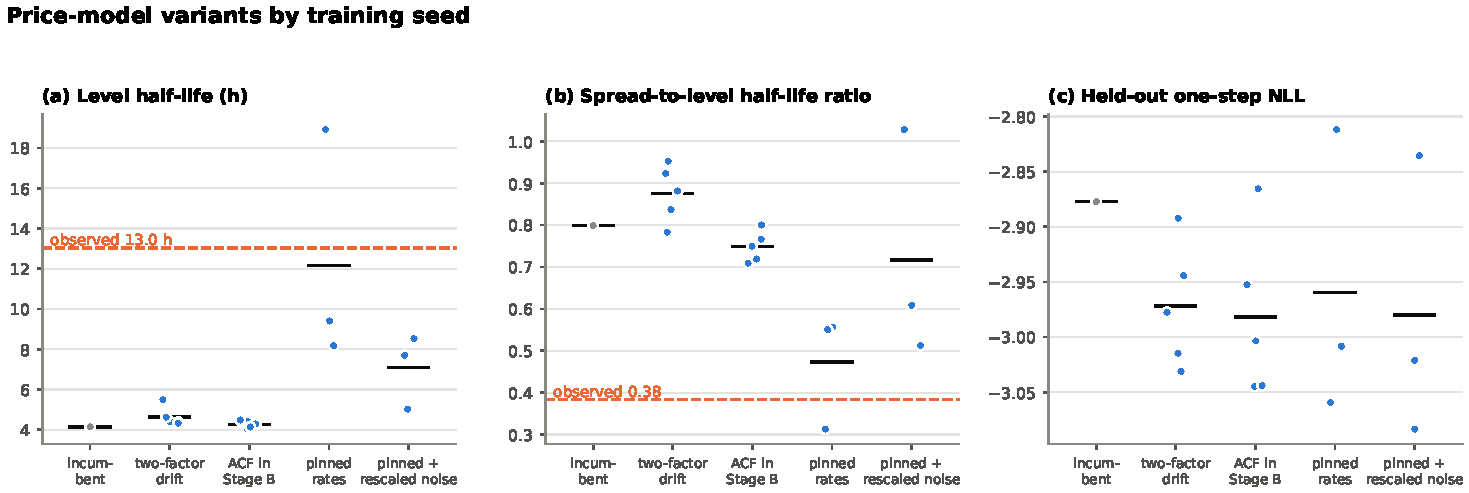
\includegraphics[width=\textwidth]{figures/twofactor_variant.pdf}
\caption{The variants of Table~\ref{tab:variants}, one dot per training
seed, with the incumbent in grey. (a)~Level half-life. (b)~Spread-to-level
half-life ratio. (c)~Held-out one-step negative log-likelihood. Dashed
lines mark the observed values.}
\label{fig:twofactor}
\end{figure}

\subsection{Cross-check residuals}

Doubling both dimensions of the DP grid left the three out-of-tolerance
points where they were, so the residual sits on the BSDE side and traces
back to the artificial SOC noise. The marginal value is read as
$Z^{(0)}/\varepsilon$, so a small $\varepsilon$ amplifies estimation
error, while a large one lets the control respond to the noise in the
state of charge and collect value from it, most of all when prices are
high. Annealing $\varepsilon$ from 8 to 2.5 during training trades the two
off. Noise crossing the kink in the clipped terminal payoff also adds
spurious Jensen value, which the linear terminal extension removes.

The three remaining points are the three smallest values in the check,
all at 10~MWh with 12 or 6 hours left. Absolute error is roughly the same
across all 60 points (mean \$195, or 2.4\% of the \$8{,}210 range of
values), and at values of \$575--2{,}000 that becomes a large relative
error.

\section{Limitations}

\paragraph{Data and market regime}
The series are day-ahead hourly trading-hub prices, not nodal or
real-time ones. The 2025--26 CAISO regime, with its large solar and
battery fleets, has compressed peaks, and conclusions about arbitrage
value are specific to it.

\paragraph{Grid model}
The congestion mechanism is shown on IEEE case14 with assigned linear
costs and one imposed thermal limit. It illustrates how congestion prices
form and is not a model of the WECC network.

\paragraph{Price model}
The simulated marginal is rejected by a block-bootstrap KS test
($p \approx 0.001$) and by the rank-histogram test, which finds the
ensemble biased high. The half-life check passes on 87.5\% of 200 seeds
for NP15 and 79.0\% for SP15, and only 73.5\% of seeds pass all fifteen
checks. The level has no long-run mean, which keeps the model usable over days to weeks but not for
multi-month unconditional simulation.

\paragraph{Control and backtest}
Jumps enter the control problem through a moment-matched diffusion, and
the viscosity regularization leaves three of the sixty cross-check states
outside the 15\% tolerance. The terminal salvage comes from the training
year's overnight prices, is far above test-quarter prices, and makes the
policy hold energy past midnight. The policy has no measurable edge over
a fixed schedule, and at three hubs a full-state grid DP is tractable, so
the deep BSDE's dimensionality advantage is never exercised. The backtest
assumes a price-taking battery with fixed efficiency ($\eta = 0.88$) and
degradation (\$2/MWh), and ignores market impact and ancillary services.

\section{Conclusion}

The neural jump-diffusion and deep BSDE policy captures 88.5\% of
perfect-foresight revenue on the test quarter. A fixed hour-of-day
schedule captures 87.5\%, and the 1.0-point gap is not distinguishable
from zero. Grid DP on the same price model ties the deep BSDE, so the
solver is not what limits the result. In a market this regular, the price
model would have to be considerably better than this one before
stochastic control could beat a schedule.

The next step is the innovation distribution: heavier-tailed increments,
or a regime-switching jump intensity, tested against the same KS and
rank-histogram criteria. The deep BSDE only becomes necessary at four or
more price nodes, where grid DP stops being tractable, so a nodal version
of the problem is the natural test for it. Real-time
co-optimization and markets with more scarcity pricing are the other
places where a stochastic controller has more room to beat a schedule.

\begin{thebibliography}{20}

\bibitem{cartea2005} Cartea, \'A. and Figueroa, M.G. (2005).
Pricing in electricity markets: a mean reverting jump diffusion model with
seasonality. \emph{Applied Mathematical Finance} 12(4), 313--335.

\bibitem{christie1993} Christie, R. (1993).
\emph{Power Systems Test Case Archive}. University of Washington,
Department of Electrical Engineering.

\bibitem{crandall1992} Crandall, M.G., Ishii, H. and Lions, P.-L. (1992).
User's guide to viscosity solutions of second order partial differential
equations. \emph{Bulletin of the American Mathematical Society} 27(1),
1--67.

\bibitem{diamond2016} Diamond, S. and Boyd, S. (2016).
CVXPY: a Python-embedded modeling language for convex optimization.
\emph{Journal of Machine Learning Research} 17(83), 1--5.

\bibitem{duffie1993} Duffie, D. and Singleton, K.J. (1993).
Simulated moments estimation of Markov models of asset prices.
\emph{Econometrica} 61(4), 929--952.

\bibitem{weinan2017} E, W., Han, J. and Jentzen, A. (2017).
Deep learning-based numerical methods for high-dimensional parabolic
partial differential equations and backward stochastic differential
equations. \emph{Communications in Mathematics and Statistics} 5(4),
349--380.

\bibitem{gneiting2007} Gneiting, T., Balabdaoui, F. and Raftery, A.E.
(2007). Probabilistic forecasts, calibration and sharpness.
\emph{Journal of the Royal Statistical Society: Series B} 69(2), 243--268.

\bibitem{hamill2001} Hamill, T.M. (2001).
Interpretation of rank histograms for verifying ensemble forecasts.
\emph{Monthly Weather Review} 129(3), 550--560.

\bibitem{hanlong2020} Han, J. and Long, J. (2020).
Convergence of the deep BSDE method for coupled FBSDEs.
\emph{Probability, Uncertainty and Quantitative Risk} 5(1), 1--33.

\bibitem{han2018} Han, J., Jentzen, A. and E, W. (2018).
Solving high-dimensional partial differential equations using deep
learning. \emph{Proceedings of the National Academy of Sciences} 115(34),
8505--8510.

\bibitem{huangfu2018} Huangfu, Q. and Hall, J.A.J. (2018).
Parallelizing the dual revised simplex method.
\emph{Mathematical Programming Computation} 10(1), 119--142.

\bibitem{kunsch1989} K\"unsch, H.R. (1989).
The jackknife and the bootstrap for general stationary observations.
\emph{The Annals of Statistics} 17(3), 1217--1241.

\bibitem{li2020} Li, X., Wong, T.-K.L., Chen, R.T.Q. and Duvenaud, D.
(2020). Scalable gradients for stochastic differential equations.
\emph{Proceedings of the 23rd International Conference on Artificial
Intelligence and Statistics}, PMLR 108, 3870--3882.

\bibitem{lucia2002} Luc\'ia, J.J. and Schwartz, E.S. (2002).
Electricity prices and power derivatives: evidence from the Nordic Power
Exchange. \emph{Review of Derivatives Research} 5(1), 5--50.

\bibitem{massey1951} Massey, F.J. (1951).
The Kolmogorov--Smirnov test for goodness of fit.
\emph{Journal of the American Statistical Association} 46(253), 68--78.

\bibitem{pardoux1990} Pardoux, E. and Peng, S. (1990).
Adapted solution of a backward stochastic differential equation.
\emph{Systems \& Control Letters} 14(1), 55--61.

\bibitem{schweppe1988} Schweppe, F.C., Caramanis, M.C., Tabors, R.D. and
Bohn, R.E. (1988). \emph{Spot Pricing of Electricity}. Kluwer Academic
Publishers, Boston.

\bibitem{sioshansi2009} Sioshansi, R., Denholm, P., Jenkin, T. and Weiss,
J. (2009). Estimating the value of electricity storage in PJM: arbitrage
and some welfare effects. \emph{Energy Economics} 31(2), 269--277.

\bibitem{thurner2018} Thurner, L., Scheidler, A., Sch\"afer, F.,
Menke, J.-H., Dollichon, J., Meier, F., Meinecke, S. and Braun, M. (2018).
pandapower: an open-source Python tool for convenient modeling, analysis
and optimization of electric power systems. \emph{IEEE Transactions on
Power Systems} 33(6), 6510--6521.

\bibitem{uhlenbeck1930} Uhlenbeck, G.E. and Ornstein, L.S. (1930).
On the theory of the Brownian motion. \emph{Physical Review} 36(5),
823--841.

\end{thebibliography}

\end{document}
